% ****************************************************************************************************
\chapter{State of the Art}\label{ch:tf}%Theoretical Foundations
% ****************************************************************************************************

%\begin{flushright}{\slshape    
	%When the wind of change blows,\\
	%some people build walls,\\
	%others build windmills.} \\ \medskip
	%--- Chinese Proverb
%\end{flushright}

Within this chapter, the theoretical foundations and related work of the thesis at hand are elucidated. At the beginning, the term business model and various points of view in regards to business models are explained. Furthermore, one business model conceptualization which is used throughout this thesis is described at the end of this section in detail. Afterwards, the concept of cloud computing, relations to other cloud computing components as well as the \ac{PaaS} domain are introduced. At the end of this chapter, related research in regards to platform strategies as well as modeling of business models is presented.

\section{Business Models}\label{ch:tf:bm}

\begin{flushright}{\slshape    
	There is nothing quite so useless,\\
	as doing with great efficiency, \\
	something that should not be done at all.} \\ \medskip
	--- Peter F. Drucker
\end{flushright}

\vspace*{-18pt}

\subsection{Origins and Definitions}

Already 1954 Peter F. Drucker proposed the five following questions in order to describe basic business strategies \citep[pp. 49-61]{Drucker1954}:

\begin{enumerate}[parsep=0pt, topsep=0pt, itemsep=0pt]
	\item What is our business?
	\item Who is the customer?
	\item What is value to the customer?
	\item What will our business be?
	\item What should it be?
\end{enumerate}

However, the term business model itself evolved noticeable within academic journals as late as during the nineties \mycite{Osterwalder2005}{pp. 3-4}{Zott2011}{p. 1022}. As of writing this paper at hand, there is no general accepted definition or uniform picture about this concept. According to \citet[p. 726]{Morris2005} and \citet[p. 1022]{Zott2011}, the term business models (at a meta level) has been referred to as an architecture, an assumption, a conceptual tool or model, a description, a design, a framework, a method, a pattern, a plan, a representation, a set, a statement, as well as a structural template. Therefore, a couple of widely used definitions with different points of view are presented below:
	
\begin{quotation}\vspace*{-5pt}{\slshape 
[A business model is] an architecture for the product, service and information flows, including a description of the various business actors and their roles; and a description of the potential benefits for the various business actors; and a description of the sources of revenues.}
\vspace*{-7pt}
\begin{flushright}
	--- \citealp[p. 2]{Timmers1998}
\end{flushright}
\end{quotation}

%\begin{quotation}\vspace*{-5pt}{\slshape 
%Business models are defined as summary of the value creation logic of an organization or a business network including assumptions about its partners, competitors and customers. They define the business and IS architecture, rules, potential benefits and the sources of revenue.}
%\vspace*{-7pt}
%\begin{flushright}
%	--- \citealp[p. 798]{Klueber2000}
%\end{flushright}
%\end{quotation}

\begin{quotation}\vspace*{-5pt}{\slshape 
A business model depicts the content, structure, and governance of transactions designed so as to create value through the exploitation of business opportunities.}
\vspace*{-7pt}
\begin{flushright}
	--- \citealp[p. 511]{Amit2001}
\end{flushright}
\end{quotation}

\begin{quotation}\vspace*{-5pt}{\slshape 
The functions of a business model are to articulate the value proposition, i.e. the value created for users by the offering based on the technology; identify a market segment, i.e. the users to whom the technology is useful and for what purpose, and specify the revenue generation mechanism(s) for the firm; define the structure of the value chain within the firm required to create and distribute the offering, and determine the complementary assets needed to support the firm's position in this chain; estimate the cost structure and profit potential of producing the offering, given the value proposition and value chain structure chosen;  describe the position of the firm within the value network linking suppliers and customers, including identification of potential complementors and competitors; [and] formulate the competitive strategy by which the innovating firm will gain and hold advantage over rivals.}
\vspace*{-7pt}
\begin{flushright}
	--- \citealp[pp. 533-534]{Chesbrough2002}
\end{flushright}
\end{quotation}

%\begin{quotation}\vspace*{-5pt}{\slshape 
%[Business models are] stories that explain how enterprises work. A good business model answers Peter Drucker's age-old questions: Who is the customer? And what does the customer value? It also answers the fundamental questions every manager must ask: How do we make money in this business? What is the underlying economic logic that explains how we can deliver value to customers at an appropriate cost?}
%\vspace*{-7pt}
%\begin{flushright}
%	--- \citealp[p. 2]{Magretta2002}
%\end{flushright}
%\end{quotation}

\begin{quotation}\vspace*{-5pt}{\slshape 
A business model is a concise representation of how an interrelated set of decision variables in the areas of venture strategy, architecture, and economics are addressed to create sustainable competitive advantage in defined markets.}
\vspace*{-7pt}
\begin{flushright}
	--- \citealp[p. 727]{Morris2005}
\end{flushright}
\end{quotation}

%\begin{quotation}\vspace*{-5pt}{\slshape 
%A business model is a conceptual tool that contains a set of elements and their relationships and allows expressing the business %logic of a specific firm. It is a description of the value a company offers to one or several segments of customers and of the architecture of the firm and its network of partners for creating, marketing, and delivering this value and relationship capital, to generate profitable and sustainable revenue streams.}
%\vspace*{-7pt}
%\begin{flushright}
%	--- \citealp[p. 10]{Osterwalder2005}
%\end{flushright}
%\end{quotation}
	
\begin{quotation}\vspace*{-5pt}{\slshape 
[A business model is] a representation of a firm's underlying core logic and strategic choices for creating and capturing value within a value network.}
\vspace*{-7pt}
\begin{flushright}
	--- \citealp[p. 202]{Shafer2005}
\end{flushright}
\end{quotation}

%\begin{quotation}\vspace*{-5pt}{\slshape 
%The particular business concept (or way of doing business) as reflected by the business's core value proposition(s) for customers; its configurated value network to provide that value, consisting of own strategic capabilities as well as other (e.g. outsourced/allianced) value networks; and its continued sustainability to reinvent itself and satisfy the multiple objectives of its various stakeholders.}
%\vspace*{-7pt}
%\begin{flushright}
%	--- \citealp[p. 40]{Voelpel2005}
%\end{flushright}
%\end{quotation}

\begin{quotation}\vspace*{-5pt}{\slshape 
A business model \ldots consists of four interlocking elements [customer value proposition, profit formula, key resources, and key processes] that, taken together, create and deliver value.}
\vspace*{-7pt}
\begin{flushright}
	--- \citealp[p. 52]{Johnson2008}
\end{flushright}
\end{quotation}

\begin{quotation}\vspace*{-5pt}{\slshape 
A business model describes the rationale of how an organization creates, delivers and captures value.}
\vspace*{-7pt}
\begin{flushright}
	--- \citealp[p. 14]{Osterwalder2010}
\end{flushright}
\end{quotation}

Most of the previously mentioned definitions of the term respectively concept business model emphasize to abstract the complexity how a company does business through the concentration on the core elements and their interdependencies. \citet[p. 91]{Magretta2002} described this as follows, \textit{"Business models describe, as a system, how the pieces of a business fit together."} Furthermore, the linkage to various actors -- partner, customer, supplier, and the like -- is emphasized by many business model definitions (\citealp[p. 2]{Timmers1998}; \citealp[pp. 533-534]{Chesbrough2002}; and \citealp[p. 202]{Shafer2005}), also referred to as value chain or value network. Whereas \citet[p. 2]{Timmers1998} explicitly mentioned the profitability (i.e. benefits) for all value chain members, \citet[pp. 533-534]{Chesbrough2002} mentioned the need to define the firm's position within the value chain. \citet[p. 727]{Morris2005} and \citet[p. 202]{Shafer2005} highlighted that business models depict decision variables respectively strategic choices and, as such, represent a firm's core logic. In contrast \citet[p. 2]{Timmers1998} defined business models as an architecture for tangible and intangible assets flows and \citet[p. 511]{Amit2001} highlighted the transactions required to do business. The definitions provided by \citet[p. 52]{Johnson2008} and \citet[p. 14]{Osterwalder2010} describe rather the big picture of business models, i.e. the rationale. \citet[p. 533-534]{Chesbrough2002} provided a comprehensive definition including the business model functions like articulation, identification, estimation, description, and formulation.

The business model is further often referred to as blueprint \mycite{Osterwalder2005}{p. 2}{Johnson2008}{p. 52}. The blueprint itself represents a simplified representation and qualifies, according to \citet[pp. 11-14]{Osterwalder2005}, to capture, visualize, understand, communicate, and share a company's business logic. Especially, for the purpose of communicating and sharing business models, a common framework or language among all stakeholders is essential to avoid misunderstandings of any kind.

The two aspects value creation and value capture are further terminologies widely used within the business model literature. Both parts are reflected in many business model definitions and conceptualizations, explicit as well as implicit (\citealp[p. 511]{Amit2001}; \citealp[pp. 533-534]{Chesbrough2002}; \citealp[p. 727]{Morris2005}; \citealp[p. 202]{Shafer2005}; \citealp[p. 12]{Chesbrough2007}; \citealp[p. 52]{Johnson2008}; \citealp[p. 14]{Osterwalder2010}; and \citealp[pp. 1019-1020]{Zott2011}). \citet[pp. 729-732]{Morris2005} identified, in alignment with \citet[pp. 49-61]{Drucker1954}, six key questions concerning basic business model components:

\begin{enumerate}[parsep=0pt, topsep=0pt, itemsep=0pt]
	\item How will the firm create value?
	\item For whom will the firm create value?
	\item What is the firm's internal source of advantage?
	\item How will the firm position itself in the marketplace?
	\item How will the firm make money?
	\item What are the entrepreneur's time, scope, and size ambitions?
\end{enumerate}

Even though the concept of business models moves towards a more mature state, just a few enterprises are able to capture their current business model in a holistic view -- including strengths and weaknesses as well as interdependencies \citep[p. 52]{Johnson2008}. This lack of knowledge represents a critical competitive factor, due to the fact that the underlying business model is not less important than the product or technology itself, in some cases even the basis for success or failure \mycite{Chesbrough2007}{p. 12}{Johnson2008}{p. 52}. According to \citet[p. 50]{Johnson2008}, \textit{"One secret to maintaining a thriving business is recognizing when it needs a fundamental change."} Among others, they described the need for a fundamental business model adjustment experienced by Hilti, a Lichtenstein-based manufacturer of high-end power tools \citep[pp. 54-57]{Johnson2008}. In the past, Hilti was selling its power tools to contractors, however facing an intensified competition and pressure on margins, for instance with low-end power tools manufacturers. For this reason, Hilti decided to change their business model from scratch in such a way that Hilti is now selling the use of its power tools for a monthly fee instead of the power tools itself.

\subsection{Conceptualization}\label{ch:sota:bmc}

Based on an analysis of definitions for business models in literature, the definition of \citet{Johnson2008} was taken as a basis for the research presented in this paper. According to \citet[p. 52]{Johnson2008}, \textit{"A business model \ldots consists of four interlocking elements that, taken together, create and deliver value"}. These four elements are denoted as follows: \ac{CVP}, profit formula, key resources and key processes. In the following, these four elements are described in detail, shortly compared with the Business Model Canvas \citep{Osterwalder2010} and other previously mentioned business model definitions, as well as discussed why the conceptualization by \citet{Johnson2008} is used for the thesis at hand.

The \ac{CVP} is considered as the most crucial part based on its main objective to satisfy customer needs. In order to understand the customer needs, the following key questions should be answered: 

\begin{enumerate}[parsep=0pt, topsep=0pt, itemsep=0pt]
	\item Who are my target customers?
	\item What is their job to be done (problem)?
	\item How can their problems be solved (offering)? 
\end{enumerate}

The interrelation between the job to be done and the corresponding offer as well as the value of the \ac{CVP} are described by  \citet[p. 52]{Johnson2008} in the following way, \textit{"The more important the job is to the customer, the lower the level of customer satisfaction with current options for getting the job done, and the better your solution is than existing alternatives at getting the job done (and, of course, the lower the price), the greater the CVP."} 
How a company is capturing value for itself based on the offering to its customers is another key element within each business model -- named here as profit formula, consisting of the sub-elements revenue model, cost structure, margin model, and resource velocity.
Assets which are essential to create and deliver the above described \ac{CVP} are summarized as key resources. According to \citet[p. 53]{Johnson2008}, these key resources include people, technology, products, facilities, equipment, channels, as well as the company's brand respectively reputation.
Processes in combination with these assets (key resources) are necessary to deliver the value proposition to the company's customers. These processes need to be efficient, repeatable, and scalable. Key processes include repeating operations -- training, development, manufacturing, budgeting, planning, sales, and services -- as well as the company's rules, metrics, and norms \citep[p. 53]{Johnson2008}.

In summary, within the business model conceptualization proposed by \citet[p. 54]{Johnson2008} the \ac{CVP} represents the value description for the target customers. The value creation and delivery is explained by the two business model elements key resources and key processes. In Table \ref{bm:concept} the business model conceptualization is graphical depicted.

%% ****************************************************************************************************
% Business Model Concept NEW
% ****************************************************************************************************
\begin{longtable}{L{\column}L{\column}L{\column}L{\column}}
	
	\toprule
	\endfirsthead
	\toprule
	\multicolumn{4}{l}{\textit{continued from previous page (\nameref{bm:concept})}}\\ 
	\midrule
	\endhead
	\midrule
	\multicolumn{4}{r}{\textit{continued on next page}}\\
	\bottomrule
	\endfoot
	\bottomrule
	\caption[Business Model Conceptualization]{Business Model Conceptualization adapted from \citet[p. 54]{Johnson2008}}
	\label{bm:concept}
	\endlastfoot
	
	\multicolumn{4}{c}{\textbf{Customer Value Proposition (CVP)}}\\ \midrule
	
	\textbf{\small Target customer} &
	\small \textbf{Job to be done} to solve an important problem or fulfill an important need for the target customer. &
	\multicolumn{2}{L{\columnT}}{\small \textbf{Offering}, which satisfies the problem or fulfills the need. This is defined not only by what is sold but also by how it's sold.} \\ \midrule

% KEY RESOURCES
\multicolumn{2}{L{\columnT}}{\textbf{Key Resources} \small needed to deliver the customer value proposition profitably. Might include:
\begin{itemize}[leftmargin=*, parsep=0pt, topsep=0pt, itemsep=0pt]
	\item \textbf{People}
	\item \textbf{Technology, products}
	\item \textbf{Equipment}
	\item \textbf{Information}
	\item \textbf{Channels}
	\item \textbf{Partnerships, alliances}
	\item \textbf{Brand}\vspace{-\baselineskip} 
\end{itemize}
} &
\multicolumn{2}{L{\columnT}}{\textbf{Key Processes} \small as well as rules, metrics, and norms, that make the profitable delivery of the customer value proposition repeatable and scalable. Might include:
\begin{itemize}[leftmargin=*, parsep=0pt, topsep=0pt, itemsep=0pt]
	\item \textbf{Processes:} design, product development, sourcing, manufacturing, marketing, hiring and training, IT
	\item \textbf{Rules and metrics:} margin requirements for investment, credit terms, lead times, supplier terms
	\item \textbf{Norms:} opportunity size needed for investment, approach to customers and channels\vspace{-\baselineskip} 
\end{itemize}} \\ \midrule

% PROFIT FORMULA
\multicolumn{4}{L{\columnF}}{\textbf{Profit Formula} \small
\begin{itemize}[leftmargin=*, parsep=0pt, topsep=0pt, itemsep=0pt]
		\item \textbf{Revenue model:} How much money can be made: price x volume. Volume can be thought of in terms of market size, purchase frequency, ancillary sales, etc.
		\item \textbf{Cost structure:} How costs are allocated: includes cost of key assets, direct costs, indirect costs, economies of scale.
		\item \textbf{Margin model:} How much each transaction should net to achieve desired profit levels. 
		\item \textbf{Resource velocity:} How quickly resources need to be used to support target volume. Includes lead times, throughput, inventory turns, asset utilization, and so on.\vspace{-\baselineskip} 
\end{itemize} 
}\\ 
\end{longtable}





Another well-known business model conceptualization respectively framework is the Business Model Canvas introduced by \citet{Osterwalder2010}. This framework consists of nine so-called business model building blocks -- namely (1) value propositions, (2) customer segments, (3) channels, (4) customer relationships, (5) key activities, (6) key resources, (7) key partners, (8) cost structure, and (9) revenue streams. Please find the proposed representation scheme in the Appendix \ref{ch:app02} (cf. Figure \ref{fig:bmc}). Another conceptualization, consisting of four central dimensions, was developed by \citet{Frankenberger2013}. The first dimension -- who -- answers the following question already proposed by \citet[pp. 49-61]{Drucker1954}, \textit{"Who is the customer?"} Second, the description of the value for the customer represent the next dimension -- what. Also this dimension is already mentioned by \citet[pp. 49-61]{Drucker1954}, \textit{"What is value to the customer?"} The third dimension describes the value creation and delivery -- how -- and answers the following question proposed by \citet[pp. 729-732]{Morris2005}, \textit{"How will the firm create value?"} And finally, the profitability of a business model is described through the fourth dimension -- why -- and answer the question mentioned by \citet[pp. 729-732]{Morris2005}, \textit{"How will the firm make money?"} These four dimensions can be found in almost all business model definitions.

In simplified terms, the bottom part of the Business Model Canvas -- cost structure and revenue streams -- deals with the value capture aspect or, in other words, why a company should perform (or is performing) the described business model. The remaining seven building blocks -- value propositions, customer segments, channels, customer relationships, key activities, key resources, and key partners -- are representing the value creation aspect. Whereas the upper left side answers the how-, the center part (value propositions) the what-, and the\linebreak 
\vspace*{-\baselineskip}
% ****************************************************************************************************
% Business Model Concept NEW
% ****************************************************************************************************
\begin{longtable}{L{\column}L{\column}L{\column}L{\column}}
	
	\toprule
	\endfirsthead
	\toprule
	\multicolumn{4}{l}{\textit{continued from previous page (\nameref{bm:concept})}}\\ 
	\midrule
	\endhead
	\midrule
	\multicolumn{4}{r}{\textit{continued on next page}}\\
	\bottomrule
	\endfoot
	\bottomrule
	\caption[Business Model Conceptualization]{Business Model Conceptualization adapted from \citet[p. 54]{Johnson2008}}
	\label{bm:concept}
	\endlastfoot
	
	\multicolumn{4}{c}{\textbf{Customer Value Proposition (CVP)}}\\ \midrule
	
	\textbf{\small Target customer} &
	\small \textbf{Job to be done} to solve an important problem or fulfill an important need for the target customer. &
	\multicolumn{2}{L{\columnT}}{\small \textbf{Offering}, which satisfies the problem or fulfills the need. This is defined not only by what is sold but also by how it's sold.} \\ \midrule

% KEY RESOURCES
\multicolumn{2}{L{\columnT}}{\textbf{Key Resources} \small needed to deliver the customer value proposition profitably. Might include:
\begin{itemize}[leftmargin=*, parsep=0pt, topsep=0pt, itemsep=0pt]
	\item \textbf{People}
	\item \textbf{Technology, products}
	\item \textbf{Equipment}
	\item \textbf{Information}
	\item \textbf{Channels}
	\item \textbf{Partnerships, alliances}
	\item \textbf{Brand}\vspace{-\baselineskip} 
\end{itemize}
} &
\multicolumn{2}{L{\columnT}}{\textbf{Key Processes} \small as well as rules, metrics, and norms, that make the profitable delivery of the customer value proposition repeatable and scalable. Might include:
\begin{itemize}[leftmargin=*, parsep=0pt, topsep=0pt, itemsep=0pt]
	\item \textbf{Processes:} design, product development, sourcing, manufacturing, marketing, hiring and training, IT
	\item \textbf{Rules and metrics:} margin requirements for investment, credit terms, lead times, supplier terms
	\item \textbf{Norms:} opportunity size needed for investment, approach to customers and channels\vspace{-\baselineskip} 
\end{itemize}} \\ \midrule

% PROFIT FORMULA
\multicolumn{4}{L{\columnF}}{\textbf{Profit Formula} \small
\begin{itemize}[leftmargin=*, parsep=0pt, topsep=0pt, itemsep=0pt]
		\item \textbf{Revenue model:} How much money can be made: price x volume. Volume can be thought of in terms of market size, purchase frequency, ancillary sales, etc.
		\item \textbf{Cost structure:} How costs are allocated: includes cost of key assets, direct costs, indirect costs, economies of scale.
		\item \textbf{Margin model:} How much each transaction should net to achieve desired profit levels. 
		\item \textbf{Resource velocity:} How quickly resources need to be used to support target volume. Includes lead times, throughput, inventory turns, asset utilization, and so on.\vspace{-\baselineskip} 
\end{itemize} 
}\\ 
\end{longtable}



 
\noindent
right side the who-question. Also the previously mentioned six basic questions concerning business models from \citet[pp. 729-732]{Morris2005} can be ascribed to the four dimensions proposed by \citet{Frankenberger2013}. Solely the sixed question -- \textit{"What are the entrepreneur's time, scope, and size ambitions?"} -- can not be easily compared with the business model conceptualizations from \citet{Johnson2008}, \citet{Osterwalder2010}, and \citet{Frankenberger2013}, due to fact that this question concerns with strategic issues, i.e. growth or speculative model. Although the above mentioned business model conceptualizations (and also the prior introduced business model definitions) differ in the total number of defined business model elements respectively questions, they can be compared. In Table \ref{tab:bmcc}, the business model elements according to \citet{Johnson2008}, \citet{Osterwalder2010}, \citet{Morris2005}, and \citet{Frankenberger2013} are exemplary opposed.

\begin{table}[t]
	\centering
	\begin{tabular}{L{.2\textwidth}L{.2\textwidth}L{.2\textwidth}L{.2\textwidth}}
			\toprule 
			\small \textbf{\citet{Johnson2008}} & \small \textbf{\citet{Osterwalder2010}} & \small \textbf{\citet{Morris2005}} & \small \textbf{\citet{Frankenberger2013}} \\ \midrule
			\small Customer Value Proposition & \small Customer Segments & \small For whom will the firm create value? & \small Who \\
				& \small Value Propositions & \small How will the firm create value? & \small What \\ \midrule
			\small Profit Formula	& \small Cost Structure &  \small How will the & \small Why\\
				& \small Revenue Streams &  \small firm make money? &\\ \midrule
			\small Key Resources & \small Key Resources & \small What is the & \small How\\
				& \small Key Partners & \small firm's internal &\\
				& \small Channels & \small source of advantage? &\\ \midrule
			\small Key Processes & \small Key Activities & \small How will the & \small How\\
				& \small Customer Relationships & \small firm position itself in the marketplace? &\\ \bottomrule
	\end{tabular}
	\caption{Business Model Conceptualization Comparison}
	\label{tab:bmcc}
\end{table}

Platform-based business models are by nature two-sided or even multi-sided business models -- in respect of the customer segments and the corresponding value propositions. Whereas the Business Model Canvas is appropriate to utilize for one-sided business models, in the domain of platform-based business models one major shortcoming restricts its utilization. In terms of \citet{Johnson2008}, each customer segment has its own problem (job to de done) and needs a corresponding offering (value proposition). Thus, it is crucial to differentiate between different customer segments in platform-based business models. The Business Model Canvas framework cannot easily be extended (the upper center and right side -- especially the two elements value proposition and customer segments) to take into account several disjoint customer segments and their corresponding value propositions. While the framework proposed by \citet{Johnson2008} can easily consider more than one customer segment, due to the fact that several \acp{CVP} -- including the customer segment (target customer) and their value proposition (offering) -- are possible.

\section{Cloud Computing}\label{ch:tf:paas}
\begin{flushright}{\slshape 
	In pioneer days they used oxen for heavy pulling,\\
	and when one ox couldn't budge a log,\\
	they didn't try to grow a larger ox.\\
	We shouldn't be trying for bigger computers,\\
	but for more systems of computers.} \\ \medskip
	--- Grace Hopper
\end{flushright}

\vspace*{-18pt}

\subsection{Origins and Definitions}

In the recent past, a new computing paradigm in the \ac{IT} industry has emerged -- cloud computing or also referred to as utility computing. Due to the fact that cloud computing is still maturing, there is up to this point no general accepted definition or even standardization, although a considerable amount of academic and applied research has been published. A well-established and widely used definition is provided by the \ac{NIST}, despite its general and broad character:

\begin{quotation}{\slshape 
Cloud computing is a model for enabling ubiquitous, convenient, on-demand network access to a shared pool of configurable computing resources (e.g., networks, servers, storage, applications, and services) that can be rapidly provisioned and released with minimal management effort or service provider interaction.}
\vspace*{-7pt}
\begin{flushright}
	--- \citealp[p. 2]{Mell2011}
\end{flushright}
\end{quotation}

Based on a comprehensive literature review of current cloud computing definitions, \citet{Vaquero2009} identified ten essential cloud characteristics -- user friendliness, virtualization, internet centric, variety of resources, automatic adaptation, scalability, resource optimization, pay per use, infrastructure \acp{SLA}, and service \acp{SLA}. Not all of these characteristics are used throughout all the investigated definitions, however, a few of them are widely accepted and led \citet{Vaquero2009} derive a minimal cloud computing definition, encompassing \textit{"scalability, pay-per-use utility model and virtualization"} \citep[p. 51]{Vaquero2009}. Besides this minimal definition, a more comprehensive consensus definition has been extracted:

\begin{quotation}{\slshape 
Clouds are a large pool of easily usable and accessible virtualized resources (such as hardware, development platforms and/or services). These resources can be dynamically reconfigured to adjust to a variable load (scale), allowing also for an optimum resource utilization. This pool of resources is typically exploited by a pay-per-use model in which guarantees are offered by the Infrastructure Provider by means of customized \acp{SLA}.}
\vspace*{-7pt}
\begin{flushright}
	--- \citealp[p. 51]{Vaquero2009}
\end{flushright}
\end{quotation}

Inherent in the concept of cloud computing are three layers (\citealp[pp. 118-119]{Iyer2010} and \citealp[pp. 2-3]{Mell2011}) -- also referred to as cloud stack (cf. Figure \ref{fig:ccs}). The \ac{SaaS} layer is the most visible layer of cloud computing for end users, since they access here the provided on-demand applications, without the need to manage or control the underlying infrastructure. Next, the \ac{PaaS} layer enables to develop and deploy applications as well as services onto cloud infrastructure. Finally, the \ac{IaaS} layer encompasses the provision of various computing resources, for instance, processing, storage, and network. In contrast to \citet[p. 50]{Armbrust2010}, in this thesis the \ac{IaaS} as well as \ac{PaaS} layer considered as two different concepts, and not as similar or indiscernible ones. 

\begin{figure}[tb]
	\centering
	% ****************************************************************************************************
% Classification Procedural Model
% ****************************************************************************************************

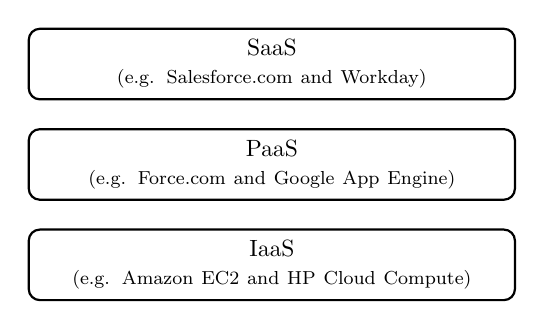
\begin{tikzpicture}[scale=0.85, every node/.style={scale=0.85}]

\node[draw,text width=20em,text centered,rectangle,rounded corners,minimum height=3em,thick] (1) at (0,3) {\acf{SaaS}\\ \footnotesize (e.g. Salesforce.com and Workday)};
\node[draw,text width=20em,text centered,rectangle,rounded corners,minimum height=3em,thick] (2) at (0,1.5) {\acf{PaaS}\\ \footnotesize (e.g. Force.com and Google App Engine)};
\node[draw,text width=20em,text centered,rectangle,rounded corners,minimum height=3em,thick] (3) at (0,0) {\acf{IaaS}\\ \footnotesize (e.g. Amazon EC2 and HP Cloud Compute)};

\end{tikzpicture}
	\caption{Cloud Computing Stack}
	\label{fig:ccs}
\end{figure}

According to \citet[p. 3]{Mell2011}, four deployment models are commonly used. First, private clouds are solely for a dedicated entity and managed by the entity itself or a third-party. Second, several entities operate together a community cloud to support a shared goal or mission. Third, public clouds are owned by an organization and open to general public or a dedicated domain. And fourth, any combination of two or more of the above mentioned clouds is denoted as a hybrid cloud.
Several authors have identified a number of features of cloud computing, which are listed below to provide a broad overview. \citet[pp. 54-58]{Armbrust2010} identified ten obstacles for cloud computing -- three concerning the adaption (availability/business continuity, data lock-in, data confidentiality and auditability), the next five affecting the growth (data transfer bottlenecks, performance unpredictability, scalable storage, bugs in large distributed systems, and scaling quickly), and the last two are business obstacles (reputation fate sharing and software licensing). \citet[pp. 120-127]{Iyer2010} described seven cloud computing capabilities -- controlled interface, location independence, sourcing independence, ubiquitous access, virtual business environments, addressability and traceability, and rapid elasticity. And finally, \citet[p. 2]{Mell2011} highlighted five essential characteristics in this field -- on-demand self-service, broad network access, resource pooling, rapid elasticity, and measured service. 

\citet{Smith2012} analyzed the cloud computing environment and reasoned that cloud computing with its various sub-concepts, like \ac{IaaS}, \ac{PaaS}, and \ac{SaaS}, is still an evolving area. However, the individual sub-concepts are at different stages of development. According to \citet[p. 5]{Smith2012}, the \ac{IaaS} and especially the \ac{SaaS} layer are already quite mature and will reach the so-called plateau of productivity in the near future. Whereas the \ac{PaaS} layer is currently at the labeled peak of inflated expectations and further research is necessary to determine the actually capabilities of this layer. Please find the complete picture of this study within Appendix \ref{ch:app03} (cf. Figure \ref{fig:cloudCycle}). Also \citet[p. 120]{Iyer2010} identified that the cloud computing area is still maturing, while the \ac{IaaS} layer is the prevalent sub-concept.

Cloud computing is especially for \acp{SME} beneficial, based on limited \ac{IT} in-house resources and knowledge associated with growing \ac{IT} requirements and needs (\citealp[p. 398]{Weinhardt2009} and \citealp{Karabek2011}). Benefits inherent in cloud computing, regardless of the customer size, are an increased flexibility, reliability, as well as agility to respond to internal and external demands (\citealp[p. 51]{Vaquero2009} and \citealp[p. 129]{Iyer2010}). Moreover, the first steps into cloud computing are not accompanied by high entry or upfront investment costs and the use of cloud computing enables companies to convert capital expenses to operating expenses (CapEx to OpEx), or, in other words, to convert fixed costs into variable costs, hence gaining the possibility to focus on their core business \citep[pp. 51-53]{Armbrust2010}. At the current state, most of the cloud computing offers are not priced based on the classical license agreements, rather on a usage-based pricing, labeled as pay as you go or pay for use pricing (\citealp[pp. 50-54]{Vaquero2009}; \citealp[pp. 51-53,58]{Armbrust2010}; and \citealp[p. 2]{Iyer2010}). A comprehensive overview about pricing strategies of software vendors is provided by \citet{Lehmann2009}.

One of the key features of cloud computing and its sub-concepts is the ability to scale according to the required demand, also referred to as elasticity (\citealp[p. 4]{Foster2008}; \citealp[pp. 52-54]{Armbrust2010}; \citealp[p. 126]{Iyer2010}; \citealp[pp. 9-10]{Zhang2010}; and \citealp[p. 2]{Mell2011}). In order to provide a flexible utilization of resources, cloud providers use the concepts of virtualization and statistical multiplexing. By using these functionalities, a cloud service can scale up nearly in real-time, hereby allocate enough resources to cope with dynamic workloads (cf. Figure \ref{fig:rpc}). In contrast to cloud services, static on-premise systems cannot easily scale dynamically and by no means in real-time. For this kind of systems a managerial decision about the expected peak load is required to determine the computing capacity necessary to perform the defined peak load. Two common cases, both suboptimal, are typical in this kind of situation. First, the peak load is underestimated and consequently the available computing capacity is not capable to handle the actual peak loads (cf. Figure \ref{fig:rpu}). And second, the peak load is overestimated and hence a large part of the computing resources is always idle, in other words, the available resources are underutilized (cf. Figure \ref{fig:rpo}). Undoubtedly, these two cases represent risks for companies -- either systems with high response times or a waste of money. The utilization of cloud services enables companies to shift these risks largely to the cloud provider and by this means staying able to act in a flexible manner.

\begin{figure}[tb]
	\centering
	\begin{subfigure}{.75\textwidth}
		\centering
		% ****************************************************************************************************
% Capacity Cloud
% ****************************************************************************************************

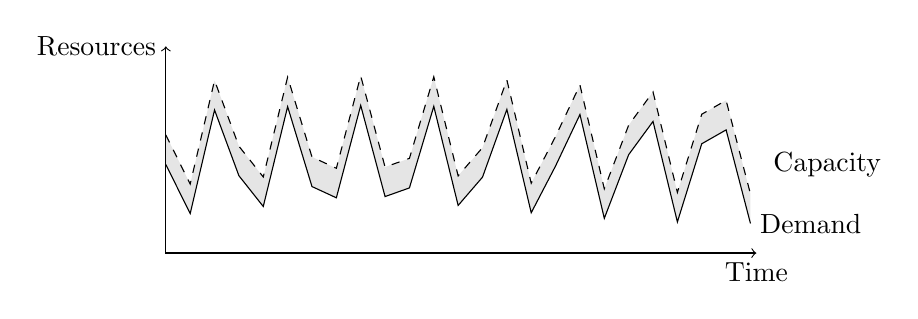
\begin{tikzpicture}[scale=0.75]

\fill[fill=gray!20] (0,1.5) -- plot [domain=0:9.9](\x, {sin(10*(\x r)) + 1.5}) -- plot[domain=9.9:0] (\x, {sin(10*(\x r)) + 2}) (0,1.5);

\draw[<->]  (10,0) node[below]{Time} -- (0,0) -- (0,3.5) node[left]{Resources};
\draw [domain=0:9.9] plot (\x, {sin(10*(\x r)) + 1.5})node[right]{Demand};
\draw [domain=0:9.9,dashed] plot (\x, {sin(10*(\x r)) + 2});
\node(1) at (11.2,1.5){Capacity};


\end{tikzpicture}



		\caption{On-Demand}\label{fig:rpc}
	\end{subfigure}
	\begin{subfigure}[b]{.75\textwidth}
		\centering
		% ****************************************************************************************************
% Capacity Static - Underprovisioning
% ****************************************************************************************************

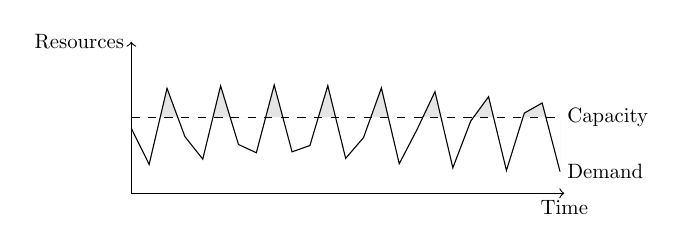
\begin{tikzpicture}[scale=0.55, every node/.style={scale=0.75}]

\fill[fill=gray!20] (0,1.75) -- plot [domain=0:9.9](\x, {sin(10*(\x r)) + 1.5}) -- (9.9,1.75) -- (0,1.75);
\fill[fill=white] (0,1.75) -- (9.9,1.75) -- (9.9,0) -- (0,0) -- (0,1.75);

\draw[<->]  (10,0) node[below]{Time} -- (0,0) -- (0,3.5) node[left]{Resources};
\draw [domain=0:9.9,dashed] (0,1.75) -- (9.9,1.75)node[right]{Capacity};
\draw [domain=0:9.9] plot (\x, {sin(10*(\x r)) + 1.5})node[right]{Demand};

\end{tikzpicture}



		\caption{Underprovisioning}\label{fig:rpu}
	\end{subfigure}
	\begin{subfigure}[b]{.75\textwidth}
		\centering
		% ****************************************************************************************************
% Capacity Static - Overprovisioning
% ****************************************************************************************************

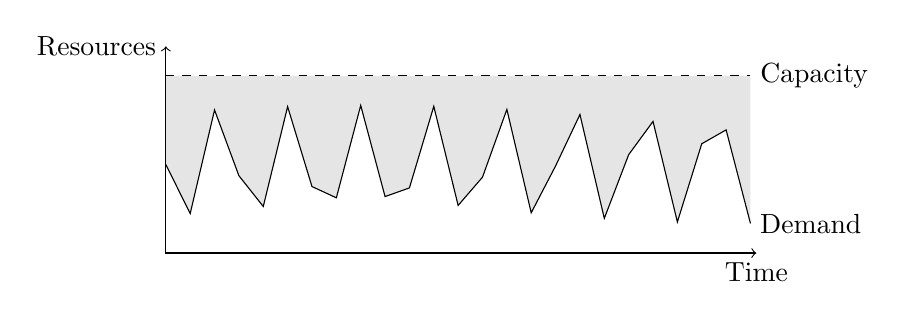
\begin{tikzpicture}[scale=0.75]

\fill[fill=gray!20] (0,3) -- plot [domain=0:9.9](\x, {sin(10*(\x r)) + 1.5}) -- (9.9,3) -- (0,3);

\draw[<->]  (10,0) node[below]{Time} -- (0,0) -- (0,3.5) node[left]{Resources};
\draw [domain=0:9.9,dashed] (0,3) -- (9.9,3)node[right]{Capacity};
\draw [domain=0:9.9] plot (\x, {sin(10*(\x r)) + 1.5})node[right]{Demand};

\end{tikzpicture}



		\caption{Overprovisioning}\label{fig:rpo}
	\end{subfigure}
	\caption[Resource Provisioning -- On-Demand vs. Static]{Resource Provisioning -- On-Demand vs. Static, adapted from \citet[p. 54]{Armbrust2010} and \citet[p. 127]{Iyer2010}}
	\label{fig:rp}
\end{figure}

\subsection{Platform as a Service}\label{ch:tf:paas:def}

For a better understanding of platforms and in particular the \ac{PaaS} layer, in the following a few more definitions are provided. These insights might be helpful in the sequel of this thesis. Product platforms are general defined by \citet{Halman2003} as follows:

\begin{quotation}{\slshape 
A platform \ldots is neither the same as an individual product, nor is it the same as a product family; it is the common basis of all individual products within a product family. \ldots The leading principle behind the platform concept is to balance the commonality potential and differentiation needs within a product family. \ldots [Therefore, product platforms are considered] as a set of subsystems and interfaces that form a common structure from which a stream of related products can be developed and produced efficiently.}
\vspace*{-7pt}
\begin{flushright}
	--- \citealp[pp. 150-151]{Halman2003}
\end{flushright}
\end{quotation}

Within the \ac{IT} industry many (technical) platforms are prevalent -- for instance operating systems (i.e. Microsoft Windows, OS X, GNU/Linux, and UNIX) and web browsers (i.e. the Mozilla Firefox web browser with diverse available add-ons). \citet{Poel2007} defined platforms within the \ac{IT} industry in the following way:

\begin{quotation}{\slshape 
[Platforms] refer to a hardware configuration, an operating system, a software framework or any other common entity on which a number of associated components or services run.}
\vspace*{-7pt}
\begin{flushright}
	--- \citealp[p. 88]{Poel2007}
\end{flushright}
\end{quotation}

Similar, but more dedicated to software platforms, \citet{Tiwana2010} defined the core concepts of these platforms as follows:

\begin{quotation}{\slshape 
[A software platform is] the extensible codebase of a software-based system that provides core functionality shared by the modules that interoperate with it and the interfaces through which they interoperate. [Whereas a module is] an add-on software subsystem that connects to the platform to add functionality to the platform. The collection of the platform and the modules specific to it [is labeled as ecosystem]. [Interfaces are] specifications and design rules that describe how the platform and modules interact and exchange information.}
\vspace*{-7pt}
\begin{flushright}
	--- \citealp[p. 676]{Tiwana2010}
\end{flushright}
\end{quotation}

Based on the above mentioned introductory platform definitions, hereafter platforms within the area of cloud computing, also known as \ac{PaaS} layer, are further defined. The first quote rather describes the \ac{PaaS} layer whereas the second one defines the \ac{PaaS} layer in general:

\begin{quotation}{\slshape 
The capability provided to the consumer is to deploy onto the cloud infrastructure consumer-created or acquired applications created using programming languages, libraries, services, and tools supported by the provider. [Footnote in the original source: This capability does not necessarily preclude the use of compatible programming languages, libraries, services, and tools from other sources.] The consumer does not manage or control the underlying cloud infrastructure including network, servers, operating systems, or storage, but has control over the deployed applications and possibly configuration settings for the application-hosting environment.}
\vspace*{-7pt}
\begin{flushright}
	--- \citealp[pp. 2-3]{Mell2011}
\end{flushright}
\end{quotation}

\begin{quotation}{\slshape
[The \ac{PaaS} layer] facilitates the development and deployment of applications without the cost and complexity of buying and managing the underlying hardware and software layers.}
\vspace*{-7pt}
\begin{flushright}
	--- \citealp[p. 178]{Marston2011}
\end{flushright}
\end{quotation}

On the basis of the five presented quotations, the concept of platforms in general as well as in the area of cloud computing should be sufficient elucidated. To sum up, \citet[pp. 150-151]{Halman2003} defined platforms in general and clarified that a platform is the basis for a several products, but still enabling these products to differentiate essentially from each other. \citet[p. 88]{Poel2007} defined platforms within the \ac{IT} industry broadly. In more detail and specially in regards to software platforms, \citet[p. 676]{Tiwana2010} defined these platforms as consisting of the core platform -- extensible codebase --, modules -- platform add-ons --, as well as an interface -- linkage between the platform and the modules. All elements together are denoted as ecosystem. A similar point of view can also be found in the definition provided by \citet[pp. 150-151]{Halman2003}. In order to use a common language and understanding of platforms, in the course of this thesis the terminology introduced by \citet{Tiwana2010} is used throughout -- platform, module, interfaces, and ecosystem.  	

\citet[pp. 2-3]{Mell2011} described the \ac{PaaS} layer as the capability to deploy acquired or self-developed applications onto cloud infrastructure, which is not managed or controlled by the \ac{PaaS} user. However the deployed application is under the user's control. Similar but with a broader scope \citet[p. 178]{Marston2011} defined the \ac{PaaS} layer encompassing the development and deployment of applications without the need to manage the underlying layers. Due to its wide character, the \ac{PaaS} definition of \citet[p. 178]{Marston2011} is used for the paper at hand. 

In simplified terms, the \ac{PaaS} layer abstracts the \ac{IaaS} layer (inclusive the automated resource management) and provides a runtime environment where applications and services run on. Usually, these software platforms are open to external developers and offer a kind of development environment, either online (i.e. browser-based) or offline (i.e. \ac{SDK}), sometimes even both variants are provided. Furthermore, these development environments address different stakeholders, ranging from technical developers to business people, and thus vary from comprehensive \acp{IDE} to graphical drag and drop environments. A powerful dashboard -- including features to administrate and manage application as well as service related issues -- completes commonly the \ac{PaaS} offer.
As mentioned earlier already, according to \citet[p. 5]{Smith2012} the \ac{PaaS} layer is currently located at the so-called peak of inflated expectations (cf. Appendix \ref{ch:app03}) and consequently some of the current \ac{PaaS} providers will be driven out of the market as well as new \ac{PaaS} providers will emerge. Furthermore, it can be expected that the competition between \ac{PaaS} providers will increase constantly. \citet[pp. 117,128-129]{Iyer2010} described those rivalry as ecosystem-based respectively network-based competiton. In the same vein, \citet[pp. 675-676]{Tiwana2010} noticed a shift of competition towards platform-centric ecosystems.

\section{Related Work/ Research}\label{ch:tf:rw}

%ca. 10 Seiten, pro Ansatz 0.5 bis 1 Seiten

\subsection{Platform Strategies}\label{ch:tf:rw:ps}

\begin{itemize}
	\item Match Your Innovation Strategy to Your Innovation Ecosystem \citep{Adner2006}
	\item Technology Strategy and Management -- The Evolution of Platform Thinking \citep{Cusumano2010}
	\item Cocreation of Value in a Platform Ecosystem: The Case of Enterprise Software \citep{Ceccagnoli2012}
\end{itemize}

\subsection{Modeling of Business Models}\label{ch:tf:rw:mbm}

\begin{itemize}
	\item USING CAUSAL LOOP DIAGRAM TO ACHIEVE A BETTER UNDERSTANDING OF E-BUSINESS MODELS \citep{Kiani2009}
	\item From Strategy to Business Models and onto Tactics \citep{Casadesus-Masanell2010}
	\item "A useful way to represent business models is by means of a causal loop diagram, where choices and consequences are linked by arrows based on causality theories" \citep[p. 198]{Casadesus-Masanell2010}
	\item Business model innovation: it's not just about technology anymore \citep{Chesbrough2007}
	\item Modeling e-business with eBML (evtl. Osterwalder 2001)
\end{itemize}